% Desarrollo
% Sergio Cuellar
% 30 de abril 2011


\chapter{Proyecto de Control de Asistencia}
\label{sec:fingerprint}

La tecnología de lectores de huellas digitales está siendo usada en una gran variedad de aplicaciones e industrias. Provee mayor seguridad y evita el mantenimiento de contraseñas. La situación actual del negocio es que las personas en los restaurantes poseen una contraseña con la cual registran su entrada, la cual les permiten comenzar a realizar operaciones el sistema punto de venta,  y salida. Las horas trabajadas son tomadas en cuenta para el cálculo de la nómina. Las contraseñas pueden ser compartidas, dando lugar a que algún compañero realice las entradas de los demás, aún cuando éstos lleguen tarde. Así mismo la salida es un problema, ya es muy común que los empleados olviden realizar su salida, y el gerente puede ingresar sus horas de salida, lo que conlleva a malentendidos. Toda esta situación afecta directamente a la nómina, ya que no se están contando de manera real las horas trabajadas.

La oportunidad de negocio consiste en poder tener la certeza de que la persona que realiza la entrada/salida es realmente ella y que no hay posibilidad de suplantar a esta persona, con lo que se tendrían ahorros significativos en gastos de nómina. Además evitar las contraseñas para usar el sistema punto de venta implica una mayor seguridad y responsabilidad en las transacciones realizadas en él.

Las huellas digitales se pueden considerar como una tarjeta de identidad visible que la naturaleza nos dio. Éstas poseen un diseño único que representan únicamente a una persona. Las huellas digitales son diminutas arrugas en la piel de nuestros dedos, tanto de las manos como de los pies, las cuales resultaron de la evolución de nuestros ancestros y cuya finalidad es la de poder sujetar de mejor manera objetos. Además sirven para poder transmitir mejor las vibraciones lo que ocasiona que se puedan distinguir las características de las superficies.

Las huellas digitales se forman de acuerdo a una combinación de la carga genética del individuo y los factores ambientales en los cuales se desarrolla, por lo que es casi imposible que el patrón de una huella digital se repita. Como consecuencia, las huellas digitales son únicas en cada individuo, incluso en gemelos. Dos huellas digitales pueden parecer iguales a simple vista, pero si se observan con más cuidado, ya sea por un investigador entrenado o un software especializado, éstos pueden encontrar las diferencias. Se les llama \textit{minutias} a las características principales de una huella digital, con las que se pueden realizar comparaciones con otras huellas. Ejemplos de minutias son, que si una arruga tiene forma de Y, de U, el abrupto final de una arruga, etc. Las minutias son los patrones que se buscan y analizan en los programas especializados en reconocimiento de huellas digitales. En la figura \ref{fig:finger_print_1} se muestra a detalle una huella digital.

\begin{figure}[htb]
 \begin{center}
  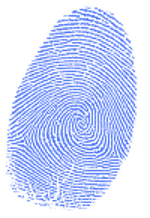
\includegraphics[scale=0.5]{fingerprint.png}
 \end{center}
 \caption{Huella Digital}
 \label{fig:finger_print_1}
\end{figure}


\section{Tipos de sensores}
\label{sec:fp_sensores}


Existen tres tipos de sensores (\textit{scanners}) de huellas digitales: ultrasónicos, ópticos y capacitivos, de los cuales los más comunes son los últimos dos.

Los scanners de huellas digitales involucran la captura de una imagen digital de la huella usando luz visible. Este tipo de sensor es en esencia una cámara digital. La capa superior del sensor, donde el dedo es colocado, se conoce como la superficie de contacto. Debajo de esta capa existe una capa que ilumina la superficie del dedo. La luz reflejada del dedo llega a un dispositivo de carga acoplada (\textit{CCD, charge-coupled device)} que captura la imagen de la huella digital. Una superficie de contacto sucia o rayada ocasiona una mala imagen de la huella digital.

Los scanners capacitivos, al igual que los ópticos, generan una imagen de la huella digital, pero en lugar de capturar la imagen mediante luz, se utiliza el principio de capacitancia. El sensor que contiene arreglos de pixeles funciona como una placa de un capacitor, la  capa de la piel, conocida como dermis (que conduce electricidad) es la otra placa, y la epidermis funciona como un dieléctrico.

\section{Ventajas y desventajas}
\label{sec:fp_pros_cons}

Existen diferentes maneras en las cuales un sistema de seguridad puede verificar que alguien es un usuario autorizado. La mayoría de los sistemas buscan por una o más de las siguientes sentencias:

\begin{itemize}
 \item Qué se tiene.
 \item Qué se sabe.
 \item Quién es.
\end{itemize}

Para entrar a un sistema tipo ''qué se tiene``, se necesita algún dispositivo como un token de autenticación, o una tarjeta RFID\footnote{Radio Frequency Identification}. Para el sistema ''qué se sabe`` se requiere que se ingrese una contraseña o un PIN. El sistema ''quién es`` busca por evidencia física de que la persona que se dice ser, es realmente ella, en esta clasificación entran las huellas digitales y el reconocimiento de voz.

Estos últimos sistemas tienen varias ventajas sobre los demás, por ejemplo:

\begin{itemize}
 \item Los atributos físicos son más difíciles de falsificar que las tarjetas de identificación.
 \item No se puede usar la fuerza bruta para adivinar una huella digital como se hace con las contraseñas.
 \item No se pueden olvidar las huellas digitales como sucede con una contraseña.
\end{itemize}

A pesar de ser tan efectivas, no son infalibles, y también tienen desventajas. Los scanners ópticos no siempre pueden distinguir bien entre la imagen de una huella digital, y una huella digital real. Y los scanners capacitivos pueden ser engañados con el molde de una huella digital. En uno de los peores casos, un criminal pudo haber cortado el dedo de una persona para poder acceder al sistema. Es por esto que algunos dispositivos ya cuentan con sensores de calor y pulso para poder distinguir estos casos.

Para hacer estos sistemas más robustos, conviene utilizar el análisis biométrico con un sistema convencional de identificación, como una contraseña. La necesidad del negocio no la requiere directamente, solamente como medio de respaldo en caso de que el dispositivo lector falle.

\section{Prototipo 1: Lector Microsoft}
\label{sec:lector_microsoft}

Al comenzar a realizar el proyecto se contaba con un lector de huellas digitales modelo ''Microsoft Fingerprint Reader``, el cual es un lector con conexión USB. La desventaja en un principio radicaba en la incertidumbre de que el dispositivo funcionara en una computadora con GNU/Linux. Al conectarlo y ejecutar el comando \texttt{dmesg} se observa que el kernel identifica correctamente el lector.

\begin{figure}[htb]
 \begin{center}
  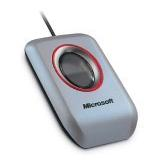
\includegraphics[scale=0.5]{microsoft_scanner.png}
 \end{center}
 \caption{Microsoft Fingerprint Reader}
 \label{fig:finger_print_2}
\end{figure}

Este lector está basado en un chipset conocido como \textit{DigitalPersona U.are.U 4000/4000B} el cual es usado en una gran cantidad de lectores, incluidos los de la compañía fabricante \textit{DigitalPersona}. El lector es del tipo óptico, el cual únicamente captura imágenes y los envía a la computadora y es necesario el uso de software para procesar y comparar las huellas digitales. Además el sensor es capaz de detectar cuando un dedo ha sido colocado o removido y se le puede indicar cuando capturar la huella digital.

Haciendo una investigación se encuentra que existe software libre que permite la lectura y procesamiento de las huellas digitales en GNU/Linux. Este software se llama \texttt{libfprint\footnote{http://www.freedesktop.org/wiki/Software/fprint/libfprint}}.  \texttt{libfprint} es una biblioteca que permite a los desarrolladores añadir soporte de lectores de huellas digitales a sus desarrollo. Algunas de sus características son:

\begin{itemize}
 \item Está escrito en lenguaje C.
 \item Depende de la biblioteca \texttt{libusb} y \textit{glib} para la comunicación.
 \item Ofrece una única interfaz de programación para la gran variedad de dispositivos que soporta.
 \item Soporta la captura y descarga en de imágenes en tiempo real desde el lector.
 \item Incluye funciones de procesamiento de imágenes.
 \item Permite el registro de huellas digitales de una persona (enrolamiento) y su verificación.
\end{itemize}

Los controladores propietarios de \textit{DigitalPersona} y su kit de desarrollo de software (SDK\footnote{Software Development Kit}) envían las imágenes cifradas a través de USB. Debido a que el método de cifrado es desconocido,  \texttt{libfprint} envía las imágenes sin esta protección. En la figura \ref{fig:finger_print_3} se muestra una huella digital adquirida por el dispositivo.

\begin{figure}[htb]
 \begin{center}
  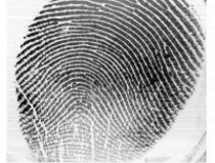
\includegraphics[scale=0.5]{fingerprint_raw_scan.png}
 \end{center}
 \caption{Ejemplo de imagen capturada por el dispositivo}
 \label{fig:finger_print_3}
\end{figure}

El lector manda una imagen de 348x289 píxeles separadas en dos transacciones, la primera es un encabezado de 64 bytes que es ignorada y después la imagen.

Uno de los grandes problemas con el sistema actual, es que a pesar de que funciona para lo que necesita hacer: tomar venta, generar reportes, etc., el sistema está sumamente desactualizado, por lo que la instalación de nuevo software puede conllevar a la actualización o instalación de nuevo software. Para la compilación del código fuente de \texttt{libfprint} se tuvo que instalar el siguiente software:

\begin{itemize}
 \item \textit{GLib} (ver. 2.28.0). Es una biblioteca de propósito general, originalmente parte de GTK+, pero a partir de la versión 2.0 los desarrolladores decidieron separarlas para crear un nuevo producto. GLib proporciona estructuras de datos avanzadas, como listas doblemente ligadas, tablas hash, arreglos dinámicos, árboles binarios, etc. Además provee de funciones para programación de hilos, colas, acceso seguro a memoria, timers, etc.
 \item \textit{ImageMagick} (ver. 6.6.0-4). Es una aplicación que sirve para crear, editar y componer imágenes. Puede leer, convertir y guardar imágenes en una gran variedad de formatos.
 \item \textit{libusb} (ver 1.0.8). Es una biblioteca que proporciona las funciones necesarias para el control en la transmisión y recepción de datos de un dispositivo USB.
 \item \textit{nss}. \textit{Network Security Services} es un conjunto de bibliotecas diseñadas por Mozilla para desarrollo de aplicaciones seguras cliente/servidor. Proporciona bibliotecas seguras como SSL\footnote{Secure Socket Layer} y S/MIME\footnote{Secure/Multipurpose Internet Mail Extensions}. Esta herramienta fue la más difícil de compilar y adaptar para el sistema actual, ya que tuve que adecuar algunos archivos del código fuente para que pudiese compilar. Además de que el código fuente que proporciona Mozilla no sigue un estándar (archivos \texttt{configure}, \texttt{Makefile} y \texttt{autoconf}) y su documentación es deficiente.
\end{itemize} 

Originalmente \texttt{libfprint} no es multiusuario, el software está diseñado para almacenar la información de las huellas digitales en el \texttt{\$HOME} de cada usuario, por lo que es necesario que los usuarios tengan una cuenta en el sistema. Para corregir este problema modifiqué el código fuente de \texttt{libfprint} con el objetivo de que se almacene la información de todos los usuarios en un solo directorio y en subdirectorios de acuerdo al número de empleado registrado en el punto de venta.

Desarrollé una interfaz gráfica usando \textit{Swing} para la entrada/salida y enrolamiento de los empleados. \textit{Swing} es una biblioteca gráfica para Java. Incluye widgets para interfaz gráfica de usuario tales como cajas de texto, botones, desplegables y tablas.

Debido a que \texttt{libfprint} está programado en C y la interfaz gráfica es en Java, utilicé JNI (\textit{Java Native Interface} para funcionar. \textit{JNI} es un framework de programación que permite que un programa escrito en Java ejecutado en la máquina virtual java (JVM) pueda interactuar con programas escritos en otros lenguajes como C, C++ y ensamblador, la desventaja más importante es la pérdida de portabilidad que ofrece Java.

Programé dos funciones en C usando JNI: la de verificación y la de enrolamiento. A continuación se muestra el encabezado del archivo de verificación:

\begin{Verbatim}
JNIEXPORT jint JNICALL Java_PRBAS_PRBAttendance_verify
  (JNIEnv *env, jobject obj, jint finger, jstring p, jstring u)
\end{Verbatim}

El apuntador \texttt{JNIEnv *env}, junto con \texttt{jobject obj} siempre deben ir al programar con JNI, ya que son interfaz con la máquina virtual de Java, después pueden ir los argumentos necesarios para la función, en este caso, \texttt{finger} que es un entero y representa al dedo a ser verificado (0-pulgar izquierdo, 1-índice izquierdo, 2-medio izquierdo, ... 9-meñique derecho), la cadena \texttt{p} indica la ruta donde se encuentra almacenada la información de las huellas digitales, y \texttt{u} es el usuario a verificar.

Una de las partes más importantes es poder ingresar al sistema punto de venta la información de entrada/salida de un empleado. No se tenía documentado exactamente cómo y dónde es que el sistema ingresa está información, por lo que tuve que revisar el código fuente para conocerlo. Para ingresar la entrada/salida el empleado debe teclear su clave en el sistema y posteriormente ingresar a las opciones de \textit{b) Entrada de Empleado} o \textit{c) Salida de Empleado}. En la figura \ref{fig:finger_print_4} se muestra la pantalla donde los asociados realizan su entrada o salida.

\begin{figure}[htb]
 \begin{center}
  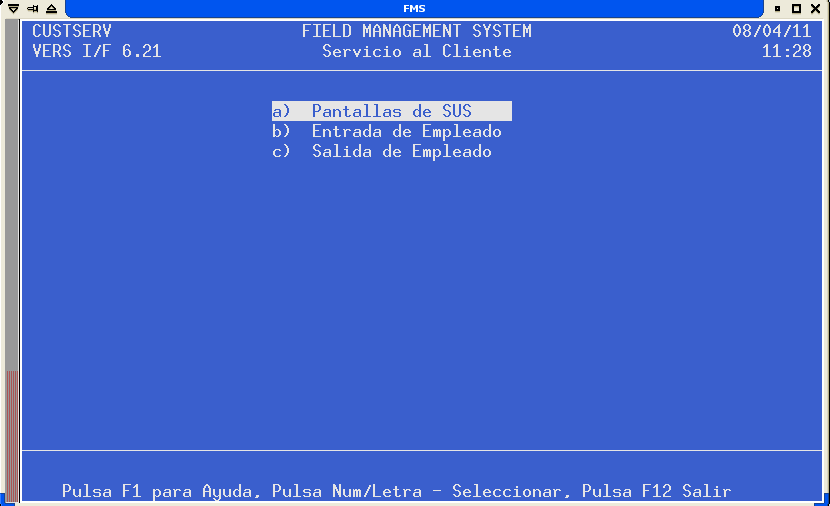
\includegraphics[scale=0.5]{fp_libfprint_fms_1.png}
 \end{center}
 \caption{Pantalla de entrada/salida en sistema punto de venta.}
 \label{fig:finger_print_4}
\end{figure}

Al realizar la entrada/salida el sistema utiliza los siguientes archivos binarios: 

\begin{enumerate}
 \item \texttt{/usr/fms/data/hrcempl.dat}
 \item \texttt{/usr/fms/data/tkeclk.dat}
 \item \texttt{/usr/fms/data/tkpaytrn.dat}
\end{enumerate}


El primero contiene los datos de todos los empleados, una línea por cada empleado: nombre, apellido, edad, dirección, etc. El siguiente archivo únicamente sirve para saber si un usuario ya registro su entrada, y contiene una copia de la línea correspondiente del archivo antes mencionado por cada usuario registrado. Y el último archivo contiene una línea por cada operación realizada de entrada y salida, identificadas con \texttt{TI} para entrada y \texttt{TO} para la salida.

El sistema punto de venta se utiliza principalmente mediante una interfaz gráfica, pero ésta se encuentra soportada por una gran cantidad de comandos que se pueden ejecutar en el shell; entre todos estos comandos, existe el comando\\ \texttt{/usr/fms/etc/sysdd} que sirve para poder poder convertir un archivo binario a texto plano, y viceversa, siempre y cuando se sepa la estructura del archivo binario. Por ejemplo, a continuación se muestra una parte de la estructura del archivo \texttt{/usr/fms/data/tkpaytrn.dat}:

\begin{Verbatim}
typedef struct  tkpaytrn_rec
{
    long    date;
    short   tran_group;
    char    fill1[2];
    char    emp_ssn[16];
    char    source;
    char    trancode[3];
\end{Verbatim}

El comando \texttt{/usr/fms/etc/sysdd} recibe de argumentos la operación a ejecutar, convertir de binario a texto es \texttt{btoa} y al contrario es \texttt{atob}. Después la estructura del archivo y al final el archivo, para este caso sería: 

\texttt{/usr/fms/etc/sysdd btoa lhs2s16cs3 /usr/fms/data/tkpaytrn.dat}

La \texttt{l} es para el tipo de dato \texttt{long}, la \texttt{h} para \texttt{short}, la \texttt{s} para arreglos \texttt{char} seguido por el número de elementos y \texttt{c} para un sólo \texttt{char}.

\begin{figure}[htb]
 \begin{center}
  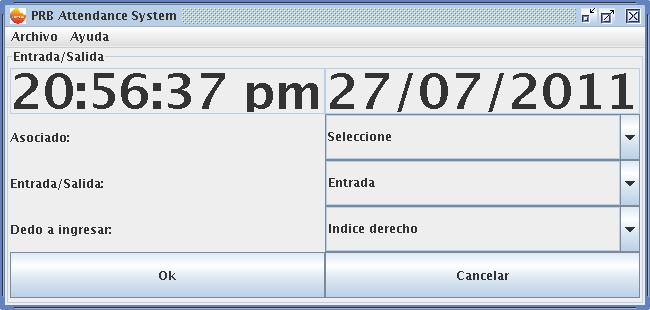
\includegraphics[scale=0.4]{fp_libfprint_attendance_1.png}
 \end{center}
 \caption{Pantalla de entrada/salida con lector de huellas digitales.}
 \label{fig:finger_print_5}
\end{figure}


En la figura \ref{fig:finger_print_5} se observa la interfaz en Swing de la aplicación de Entrada/Salida. Como se puede observar, ésta cuenta con la fecha y hora actual, con la cual se almacenará el registro. Al seleccionar el asociado se muestra una lista de todos los empleados registrados en el sistema punto de venta, los cuales son extraídos a través de comandos de SUS. En la figura \ref{fig:finger_print_6} se muestra el despliegue de la lista de asociados.

\begin{figure}[htb]
 \begin{center}
  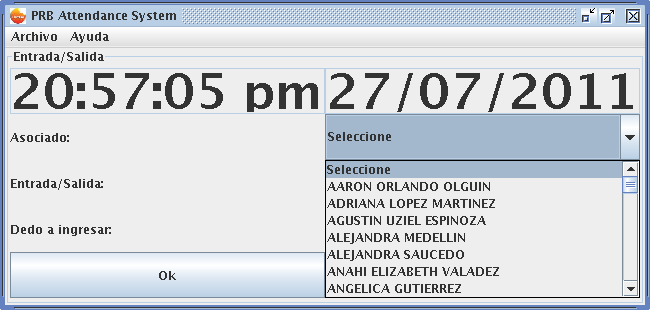
\includegraphics[scale=0.4]{fp_libfprint_attendance_2.png}
 \end{center}
 \caption{Listado de asociados.}
 \label{fig:finger_print_6}
\end{figure}

La selección de entrada/salida sirve para ingresar \texttt{TI} o \texttt{TO} en el archivo correspondiente. Un área de oportunidad en el desarrollo es la detección automática si es entrada o salida. Lo que sí debe ser seleccionado, debido a la naturaleza de la biblioteca \texttt{libfprint}, es la selección del dedo de la huella digital a ingresar. Esto se debe a que el software no es capaz de realizar la comparación entre todas las huellas digitales almacenadas de un mismo usuario, y mucho menos de realizar esta comparación para las huellas de todos los usuarios. Por lo que se le debe decir el usuario y el dedo a ingresar, para que el software únicamente haga la comparación de la huella a verificar y la que fue previamente almacenada. Al dar click en \texttt{OK}, se solicita al usuario que coloque el dedo correspondiente en el lector de huellas digitales, se recomienda colocarlo por alrededor de 3 segundos y retirarlo; el lector, como se mencionó anteriormente, es capaz de detectar la colocación  y remoción de un dedo. En caso de que no se haya verificado la huella digital, la interfaz solicitará que se vuelva a colocar el dedo. Esta interfaz aparece una vez que el usuario ha seleccionado la opción correspondiente (\texttt{b)} o \texttt{c)} de la figura \ref{fig:finger_print_4}).

Para el almacenamiento de las huellas digitales o el enrolamiento, se utiliza una interfaz más simple, en la cual únicamente se selecciona el usuario y el dedo. El procedimiento al hacer click en \texttt{OK} es el mismo que en la verificación. Por razones de seguridad y de evitar el múltiple enrolamiento de una misma huella digital para diferentes usuarios, esta funcionalidad se activa a petición del gerente del restaurante.

Es importante mencionar, que la biblioteca \texttt{libfprint} es capaz de obtener una fotografía de la huella digital, ésta no es utilizada para el análisis de las minutias, \texttt{libfprint} genera un archivo de datos binarios, el cual no puede ser leído por un editor de textos. La imagen de la huella digital es eliminada, ya que de acuerdo a la nueva \textit{Ley de Protección de Datos Personales en Posesión de los Particulares} se debe tener un mayor cuidado en el manejo en este tipo de datos para no caer en problemas legales.

Es por esto que busqué un dispositivo más especializado, el cual se describe con más detalle en la sección \ref{sec:lector_zksoftware}.

En las pruebas realizadas en este dispositivo observé que la verificación exitosa depende de la forma en que se haya capturado la huella digital en el enrolamiento. Debido a que el software únicamente usa una sola huella digital para obtener las minutias, al colocar de otra forma el dedo, ocasiona que muchas minutias no correspondan y arroje como resultado que la huella digital no corresponde. Esto ocasionaría un enorme problema en los restaurantes, elevando el número de soportes técnicos diariamente debido a que los empleados no pueden registrar su entrada ni entrar al sistema.

\section{Prototipo 2: Lector ZK Software}
\label{sec:lector_zksoftware}

Existen en el mercado una gran variedad de dispositivos lectores de huella digitales, que además de almacenarlas y verificarlas, son capaces de generar diversos reportes de acuerdo a la información de sus registros utilizando software externo o dentro del dispositivo. Una de las principales características que deben tener los lectores para poder integrarlos fácilmente al sistema en el restaurante, es que se puedan descargar los registros a la computadora sin tener un software intermediario, el cual siempre es para Windows. 

Encontré el lector de huellas digitales de la compañía ZK Software modelo U300 (ver figura \ref{fig:finger_print_7}) el cual cuenta con un puerto Ethernet RJ45 y USB. Es capaz de almacenar 1600 huellas digitales, 50000 registros, tiene sistema operativo GNU/Linux.

\begin{figure}[htb]
 \begin{center}
  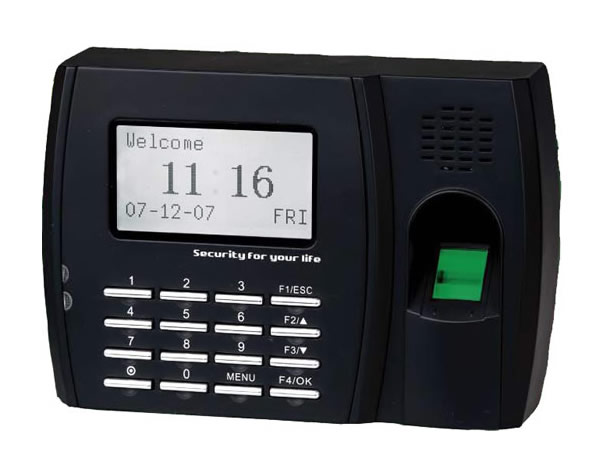
\includegraphics[scale=0.4]{fingerprint_u300.png}
 \end{center}
 \caption{Lector de huellas digitales U300 de ZKSoftware}
 \label{fig:finger_print_7}
\end{figure}

Una de las principales características de este lector, es que una vez configurada su dirección IP, se puede acceder a una página web para consultar los registros almacenados como se muestra en la figura \ref{fig:finger_print_8}. Se pueden obtener registros del día actual, de ayer, de la semana pasada, o bien especificar la fecha para desplegarlos. 

\begin{figure}[htb]
 \begin{center}
  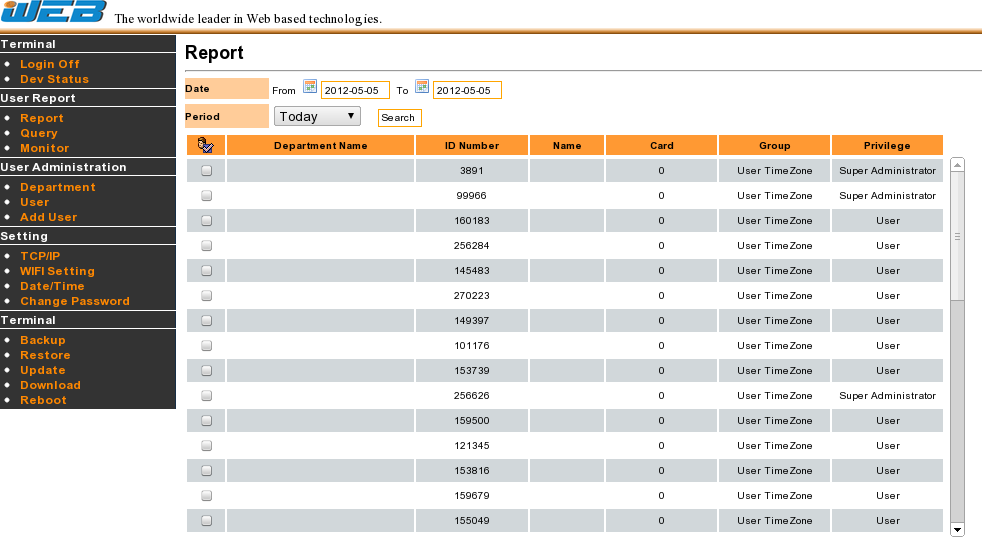
\includegraphics[scale=0.4]{fingerprint_web_new_1.png}
 \end{center}
 \caption{Página web del dispositivo mostrando usuarios registrados.}
 \label{fig:finger_print_8}
\end{figure}

El procedimiento para obtener los datos y el registro de los empleados es el siguiente:

\begin{enumerate}
 \item Mediante cURL\footnote{cURL es una herramienta para usar en un intérprete de comandos para transferir archivos con sintaxis URL, soporta FTP, FTPS, HTTP, HTTPS, TFTP, SCP, SFTP, Telnet, DICT, FILE y LDAP.} se debe obtener la cookie de la página web del lector de huellas digitales, para poder consultar los registros.
 \item Con la cookie previamente descargada y con cURL se accede a la dirección \url{http://192.168.101.23/csl/report}. En este caso la IP del lector de huellas es \texttt{192.168.101.23}. Con esto se obtiene la imagen de la figura \ref{fig:finger_print_8} que sirve para obtener los números de empleados de los usuarios registrados.
 \item Con cada uno de los números de empleados obtenidos en el punto anterior, se consulta con cURL el URL \url{http://192.168.101.23/action=run&sdate=2012-02-20&edate=2012-02-20&uid=23021} con la fecha inicial y final igual para obtener el día especificado, además del número de empleado con el que se registro, de esta manera se obtiene la página con los registros almacendados para ese usuario. En caso de que el usuario no tenga registros para ese día, se pasa al siguiente usuario.
 
 \begin{figure}[htb]
 \begin{center}
  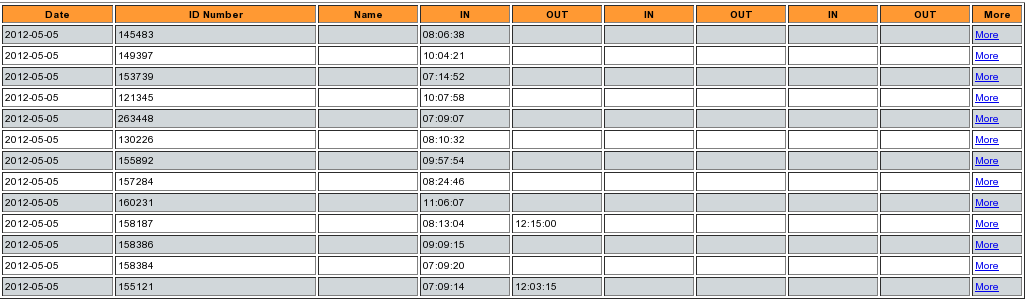
\includegraphics[scale=0.6]{fingerprint_web_new_2.png}
 \end{center}
 \caption{Página web mostrando los registro en un día específico.}
 \label{fig:finger_print_9}
\end{figure}
 
 \item Con ayuda de Perl y el módulo \texttt{HTML::TableExtract} se parsea la página HTML obtenida en el punto anterior y se obtiene principalmente, la columna de hora. Se parsean todas los renglones de hora que existan. Por lo menos debe existir un registro de hora, la cual se considera la entrada.
 \item Con el ID del usuario, la fecha y la hora de entrada y/o salida, se realiza una consulta a la base de datos de PostgreSQL para revisar si no ha habido registro de este usuario.
 \begin{itemize}
  \item Si tiene un registro de hora, es su entrada, se registra en base de datos y en los archivos necesarios en el punto de venta.
  \item Si tiene dos registros de hora, es su salida, y se registra en la tabla de la base de datos y se actualizan los archivos correspondientes del punto de venta.
  \item Existe una opción de configuración en el lector biométrico en donde se establece el tiempo mínimo en el que puede registrar otro evento. Éste parámetro se estableció en cuarenta y cinco minutos. Durante la primera fase de pruebas se desconocía este parámetro y se observaba que los usuarios hacían un uso incorrecto del lector, colocando más de una vez su dedo en un lapso muy corto de tiempo, por lo que se tenían muchos registros innecesarios.
 \end{itemize}

\end{enumerate}

\subsection{Descripción de scripts}
\label{sec:desc_scripts_finger}

A continuación se describen a grandes rasgos los scripts involucrados en todo el proceso de registro:

\begin{itemize}
 \item \texttt{getFPdata.sh}: Mediante este script, que es ejecutado mediante un cron, se realiza todo el proceso de registro. Recibe de parámetro la fecha a procesar. Dentro de este script obtienen mediante \texttt{getIDs.pl} los números de empleado que se tienen registrados. Con estos números de empleado se realizan consultas a sus registros mediante \texttt{parseHours.pl}.
 \item \texttt{getIDs.pl}: Es el encargado de obtener los números de empleado registrados. Pero además de los números de empleado, obtiene los valores de los \textit{checkboxes} que se muestran en la figura \ref{fig:finger_print_8} para poder hacer las consultas respectivas.
 \item \texttt{parseHours.pl}: Con él se obtienen, en caso de tener, los registros de entrada/salida de cada empleado, así como la inserción o actualización en la tabla de PostgreSQL \texttt{pp\_emp\_check} y el registro de las horas en los archivos del sistema de punto de venta.
 \item \texttt{clock\_employee.sh}: Realiza el registro en los archivos punto de venta para que puedan ser analizados por los procesos de nómina.
\end{itemize}

El script \texttt{getFPdata.sh} se lleva a cabo en un proceso CRON cada cinco minutos. Lo que garantiza que una vez que el usuario ha realizado su verificación en el lector, éste pueda utilizar de manera casi inmediata el sistema punto de venta.  No todos los usuarios utilizan directamente las terminales, el único puesto que maneja directamente las terminales son las personas que atienden los destinos de servicio a domicilio y auto (este destino es aquel en que el cliente ingresa con su carro al estacionamiento y realiza la orden desde él); por lo que se ejecute cada cinco minutos el proceso que lee y procesa los datos del lector es correcto para la operación.

Además elaboré unos scripts para monitorear que el dispositivo se encuentre conectado a la red y pueda mandar correos electrónicos dirigidos al gerente del restaurante y de área para que estén enterados de la perdida de comunicación del lector por alguna causa.

El gerente del restaurante no tiene acceso a la página web del lector biométrico, por lo que para que pueda visualizar los registros de una manera rápida y fácil desarrollé el reporte titulado ''Reporte de Asistencias en Biométrico`` dentro de eReports, donde puede seleccionar una fecha para poder conocer los horarios en que laboró cada empleado y poder cotejar con la nómina de cada semana, que ésta sea correcta.

 \begin{figure}[htb]
 \begin{center}
  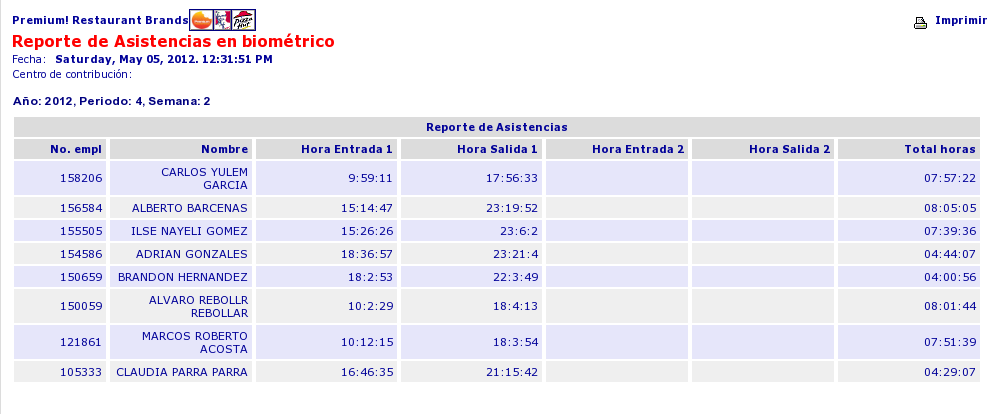
\includegraphics[scale=0.6]{fingerprint_ereports.png}
 \end{center}
 \caption{Reporte de asistencia en eReports.}
 \label{fig:finger_print_ereports}
\end{figure}

A la fecha el desarrollo ya se encuentra funcionando al 100\% y en prueba en dos restaurantes, no se ha liberado a más centros debido a que el área de Operaciones y Legal debe realizar adecuaciones a los contratos actuales, así como la de elaborar un plan de entrenamiento a los empleados por parte del área de Entrenamiento con asesoría de Operaciones y Desarrollo a Restaurantes.

Es muy importante que en el momento del enrolamiento o la verificación se coloque de manera adecuada el dedo, ya que de otra manera, existirán errores de captura/lectura. La correcta forma de colocar el dedo en el centro del lector de una manera plana y firme como se muestra en la figura \ref{fig:finger_print_10}.

\begin{figure}[htb]
 \begin{center}
  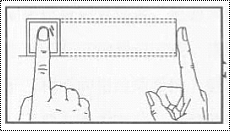
\includegraphics[scale=0.7]{place_finger_1.png}
 \end{center}
 \caption{Forma ideal para colocar el dedo en el lector.}
 \label{fig:finger_print_10}
\end{figure}

Es considerada una mala colocación del dedo en el lector, cuando el dedo no se encuentra completamente plano, no se encuentra en el centro del lector, ya sea que esté muy a la derecha, izquierda o abajo. O cuando el dedo no haga contacto la huella digital con el lector como se muestra en la figura \ref{fig:finger_print_11}.

\begin{figure}[htb]
 \begin{center}
  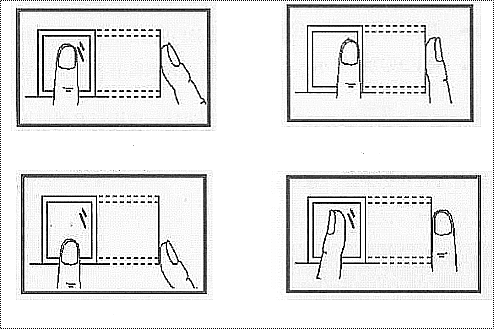
\includegraphics[scale=0.7]{place_finger_2.png}
 \end{center}
 \caption{Forma incorrectas para colocar el dedo en el lector.}
 \label{fig:finger_print_11}
\end{figure}